%\documentclass[aps,prrd,preprint]{revtex4}
\documentclass[aps,prd,final,onecolumn,a4paper,10pt]{revtex4}

% Note:  comment out one of the two documentclass commands, depending
% on whether you need the final or preprint version. It is most convenient
% to work in preprint mode, and switch to final only at the end.
\usepackage{float}
\usepackage{graphicx}                            % Graphics package
\usepackage{amsmath}
\usepackage{verbatim}
\usepackage[margin=1in]{geometry}
\usepackage{subcaption}

\captionsetup{compatibility=false}


\DeclareMathOperator*{\argmin}{arg\,min}

\begin{document}

\title{6.872 Final Report}
\author{Iris Xu , Dalesh S Dharamshi }	
\date{\today} 

\begin{abstract}
\noindent
  In the era of personalized medicine it is anticipated that an individual patient's health record will contain multiple molecular expression profiles that have been captured across multiple time points in various health states. Accurate identification \& representation of changes in molecular expression patterns across time and linking them to potential health conditions is at the core of the effectiveness of personalized medicine. 
  
  We introduce sequence alignment score driven clustering to accurately identify changes in molecular expression over time , this approach can group time-shifted expression signals that may have a causal relationship.
  
  We further provide a concept of visualizing these clusters of change in molecular expression across time along with annotations of various health and biologically relevant terms enriched for each cluster.
  
  Our results indicate that using alignment score as a distance to clustering produces clusters that includes signals that may have time shifted due to an upstream or downstream relation.These signals tend to be separated into different clusters while using the standard UPGMA based clustering. 
  Of the three time course datasets we tried this approach, only two of them appear to show a corresponding enrichment of biological terms associated with the identified clusters. The root cause for the failure for clusters to show significant enrichment in the third dataset is yet to be identified.
  Our visualzation provide an overview of changes represented by our gene clusters. However, fetching in real-time from DAVID web service, ENSEMBL, and OMIM is slow and makes real-time visualization of these annotations difficult.
  
\end{abstract}

\maketitle

\pagestyle{myheadings}
\markboth{!!!?!}{6.872 Final Report}
\thispagestyle{empty}

%%%%%%%%%%%%%%%%%%%%%%%%%%%%%%%%%%%

\section{Background}
	\begin{figure}[H]
\centering
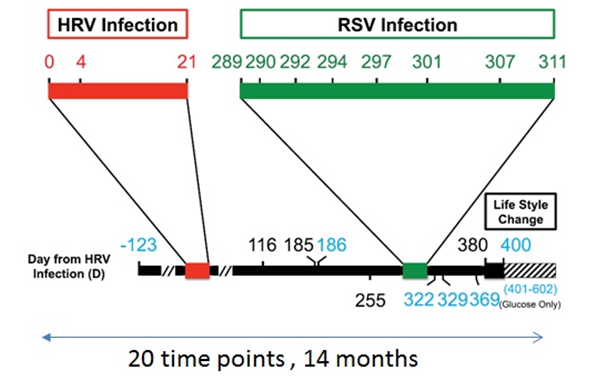
\includegraphics[scale=0.65]{Introduction.png}
\caption{An individual patients molecular profile captured across time points.}
\label{fig:PatientTimeCourses}
\end{figure}

	In the era of personalized medicine it is anticipated that an individual patient's health record will contain multiple molecular expression profiles that have been captured across multiple time points in various health states. Accurate identification \& representation of changes in molecular expression patterns across time and linking them to potential health conditions is at the core of the effectiveness of personalized medicine.Additionally, a patient is likely to have more than one health condition being expressed at the same time.

  Unlike a test for differential gene expression in one or more conditions, the clinical setting described above has the additional complexity of analyzing a time course of multiple biological components sampled across disparate time points and health conditions. The challenge is providing a concise description of an individual’s state that can be easily analyzed in this clinical setting. We investigate a few aspects of this complexity in order to facilitate generating a clinical recommendation.

  While previous work has focused on monitoring and grouping molecular expression along the gene or conditions axes to identify changes , our goal is to introduce alignment to potentially improve the accuracy of this grouping by including potentially time-shifted signals that may have a relation. 
  In addition we intend to arrive at a visual overview of the change in an individual’s health state by identifying, separating, and annotating related biological component groups that have similar changes in expression levels, potentially time-shifted indicating a potential causal relationship.
  
  Note : That we did our project as a combined work between two of our classes 6.872 and 6.878.

\section{Results and Discussion}
\subsection{Input dataset and Preprocessing}
\begin{description}
 \item 1. GSE33029 : "Integrated analysis of omics profiles"
 
 We have primarily used this ‘Snyderome’ dataset which contains various molecular expression captured across 20 time points over 14 months for a single individual.

The RNASeq dataset ( ~120 gb ) posted on GEO is the output of topHat and we had to perform the following preprocessing.
\begin{description}
 \item a. Cufflinks analysis to derive gene expression abundance in FPKMs
 \item b. Filtering,Quantile normalization,vector normalization of the cufflinks output.
 \item c. We then created multiple views of this expression data to get a feel for how the
		data looks.
\end{description}


In addition to the above we tested our methodology on the following two time course gene expression datasets available on GEO. No additional preprocessing was done to these datasets.

 \item 2. GSE19392 "Dynamic responses of primary human bronchial epithelial cells to influenza virus, viral RNA and interferon-beta"
 \item 3. GSE675 Time course analysis of response to HCMV infection
\end{description}


\subsection{Alignment}

The goal of our project was to find genes with similar expression patterns, indicating potential biological relevance.
In order to first find a measure of similarity, we calculated a distance metric between series using alignment.
We wanted similar expression signals to have a smaller distance. In particular, we wanted to capture the fact that changes in expression of one gene may affect the expression of another gene, but in the future. Additionally, we wanted to capture that the upregulation of a gene may cause the downregulation of another gene.
\\

Each processed gene expression series was converted to a character string.
We set a threshold change level, initally at $10$ percent.
If the expression level increased by more than the threshold from the previous timepoint, we convert to an \verb!R! for Rise.
If it decreased by more than the threshold, we convert to a \verb!D! for Drop.
And if it did not change by more than the threshold level, we convert to \verb!S! for Steady. The first character is always \verb!S!.\\

For example, the sequence $10$, $100$, $8$, $11$, $10$ is converted to \verb!S!, \verb!D!, \verb!R!, \verb!S!. Sequences were aligned and scored using Needleman-Wunsch.
In order to potentially align signals that have similar but negative expressions of each other, we attempted to give a smaller mismatch penalty between \verb!R! and \verb!D!. We also tried stricter versions of the scoring matrix to allow softened mismatch (between steady and anything else) or no mismatches (Table \ref{tab:scoring}).
We also varied the gap penalty depending on how far apart the time points were. For very far apart signals, we used a larger penalty.
While sequence alignment is polynomial, we aligned on the order of $10^5$ sequences, so we modified our inital sequence alignment implementation to include gap penalty lookup as a speedup.
Alignment was run on a combination of AWS nodes and the Broad cluster.

\begin{table}[H]
\caption{Some sample scoring matrices alignment: least strict (allowing matches between drops and rises in signal for potention downregulation effects), more strict (giving mismatches between rises and drops), most strict (penalizing mismatches). The gap penalty depends on the time offset between two time points, increasing with time differences.}
\label{tab:scoring}
\begin{center}
\begin{tabular}{c | ccc}
  & R & D & S\\ \hline

  R &  3 & -1 & -3\\
  D & -1 & 3 & -3\\
  S & -3 & -3 & 1\\
\end{tabular}
\quad
\begin{tabular}{c | ccc}
  & R & D & S\\ \hline

  R &  3 & -3 & -1\\
  D & -3 & 3 & -1\\
  S & -1 & -1 & 3\\
\end{tabular}
\quad
\begin{tabular}{c | ccc}
  & R & D & S\\ \hline

  R &  3 & -3 & -3\\
  D & -3 & 3 & -3\\
  S & -3 & -3 & 3\\
\end{tabular}
\end{center}
\end{table}

\subsection{Clustering}


Given the distance matrix generated by alignment, we were able to cluster similar sequences.
Our clustering was based on the alignment scores generated above as distance.
One question that needed to be resolved was how determine the optimal number of
clusters.We have tried the following two approaches towards this
a. Pairwise clustering until we reach a threshold of the alignment score between
two clusters.
b. Affinity propagation based clustering to automatically determine the number of
clusters.The pairwise heirarchical clustering with an emperical value of threshold based
out of experiments gives us fewer clusters than the affinity propogation . However the clusters 
generated by affinity propogation appear to be more cohesive.

We compared our clustering and alignment to the standard UPGMA clustering. We generated a heirarchical clustering output on the same preprocessed dataset with the help of an external tool ‘Cluster 3.0’ developed by Michael Eisen at stanford.
Shown below are three heatmaps the first two heatmaps are from clusters generated by our implementation of alignment and clustering (affinity prop followed by heirarchical) the third generated by cluster 3.0. In yellow is an example of a cluster that based on the signal appears to belong together but is spread out in multiple clusters if alignment is not considered for clustering.

\begin{figure}[H]
\centering
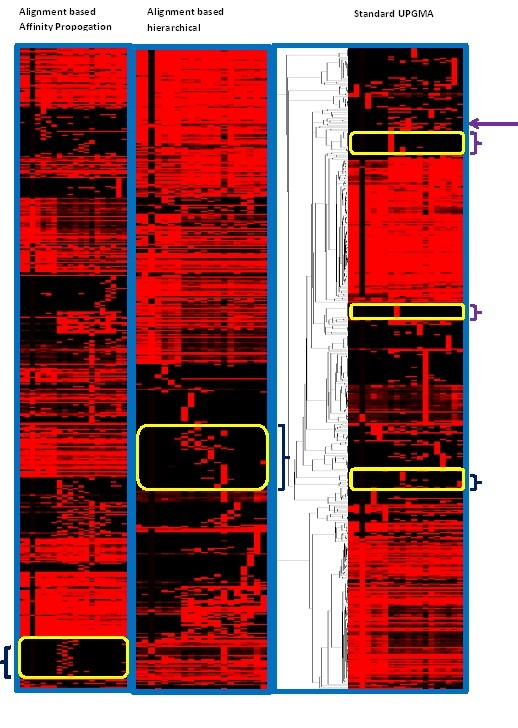
\includegraphics[scale=0.75]{ClustercomparisonResults_v2.png}
\caption{Heatmap showing the comparison of aligned clustering and UPGMA.}
\label{fig:ClusterComparison}
\end{figure}


\subsection{Enrichment Analysis}
After identifying clusters, we wanted a way to efficiently describe each cluster, as well as to measure the effectiveness of our alignment and clustering algorithm.

To analyze the efficacy of alignment in clustering, we used multiple approaches 1. Fischer's Exact test for Gene Ontology annotations. 2. We ran the gene list generated by our clusters through DAVID functional annotation tool.
Gerald Quon provided us with an \verb!R! script and Gene Ontology data for annotation testing of our clusters.

While, visually, the clusters showed alignment for GSE33029 dataset , the p-value matrices indicated no significant enrichment in our clusters after correcting for multiple comparisions with the Benjamini-Hochberg procedure. However, in order to get some quantitative measure of performance, we took sums of the p-value matrices generated from enrichment analysis for our technique for the GSE675 dataset and normalized over the same value for clusters generated by k-means. It shows that, to some degree, our alignment and clustering technique performs better than without alignment.\\

To further check if our approach works we decided to rerun our analysis on two additional and independent timecourse datasets from GEO (GSE19392 GSE675). With clusters generated from these datasets we do see significant enrichment numbers showing up for pathways and other annotation terms. The KEGG pathway results for a few of our clusters on the above datasets are as shown below. We havent yet related these results to the context of the original studies. Additional time is needed though to accurately conclude on the Enrichment analysis to pinpoint the cause for the lack of enrichment annotations for our clusters on the GSE33029 dataset.We suspected that we are missing a noise correction step for the GSE33029 dataset that may be resulting in no enrichment showing up and reanalyzed with additional normalizations in no vain. We also suspect the authors may have not fully specified the steps they took to preprocessing this dataset and we may be missing some correction step.


\begin{figure}[H]
\centering
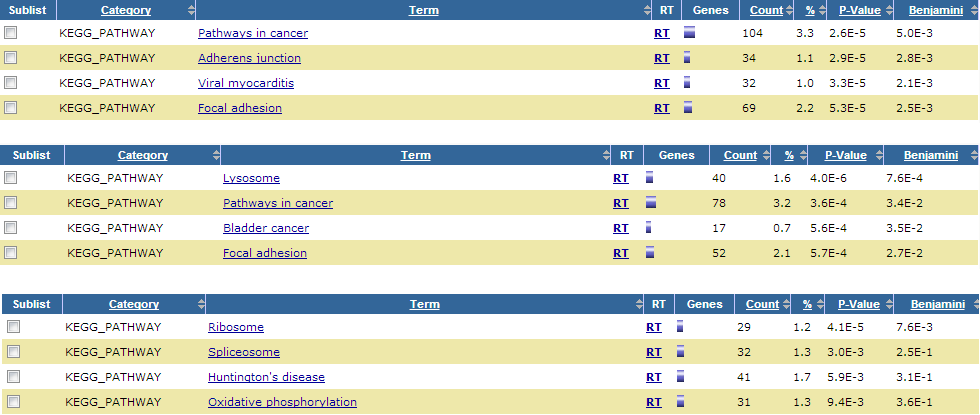
\includegraphics[scale=0.65]{3Clusters_PathwayCombined.png}
\caption{KEGG Pathway analysis on 3 clusters from GSE19392 dataset using david.}
\label{fig:KEGGPathway.}
\end{figure}



In order to provide a summarizing description of learned clusters we wanted to provide a word cloud, we initially pulled gene information from the \verb!OMIM! database. However, the text was too general even after multiple round of filtering and the generated word clouds were too non-descriptive.

We then used \verb!DAVID! Bioinformatics Database web service to find functional groups within each cluster, as a means of describing each cluster, with $kappa=70$ and $linkage = 0.50$. We were able to generate functional groups for several clusters.
The \verb!DAVID! clustering provided functional groups within each cluster, whereas corrected Fischer's Exact test tries to summarize an entire cluster. Since we were able to find significant groups within each cluster, but not for an entire cluster, this may indicate that our clustering is too general or that the clusters are too large.

\begin{figure}[h]

\end{figure}


\begin{figure}[H]
  \centering
  \begin{subfigure}[b]{0.5\textwidth}
    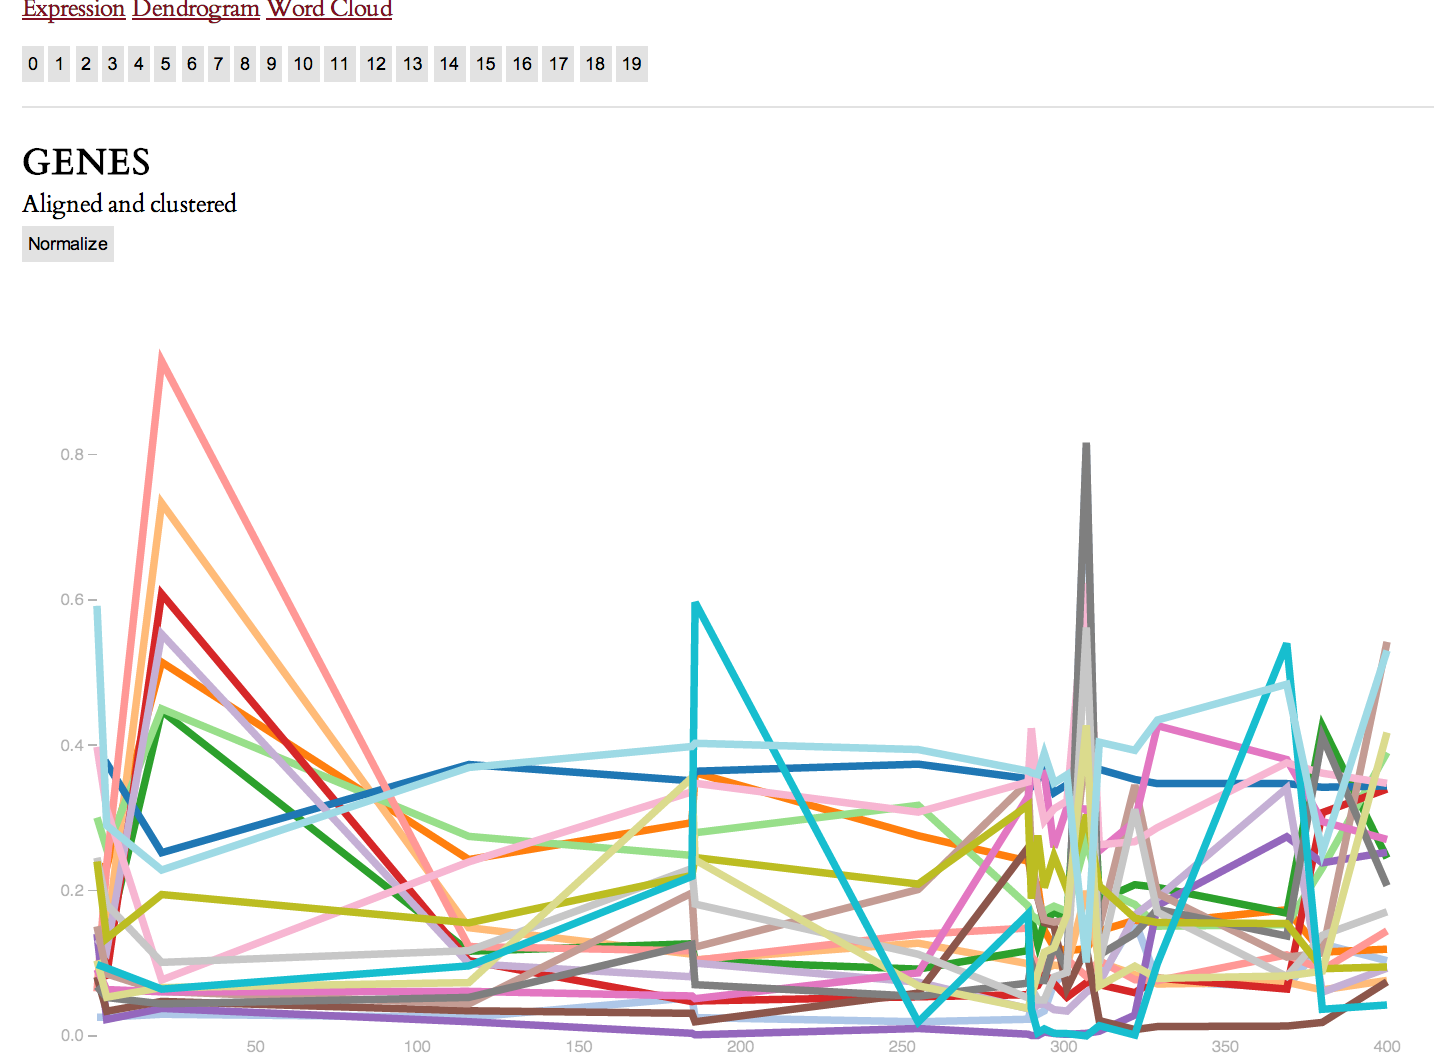
\includegraphics[width=.9\textwidth]{graphs.png}
    \label{fig:dendrogram}
  \end{subfigure}%
  ~
  \begin{subfigure}[b]{0.5\textwidth}
    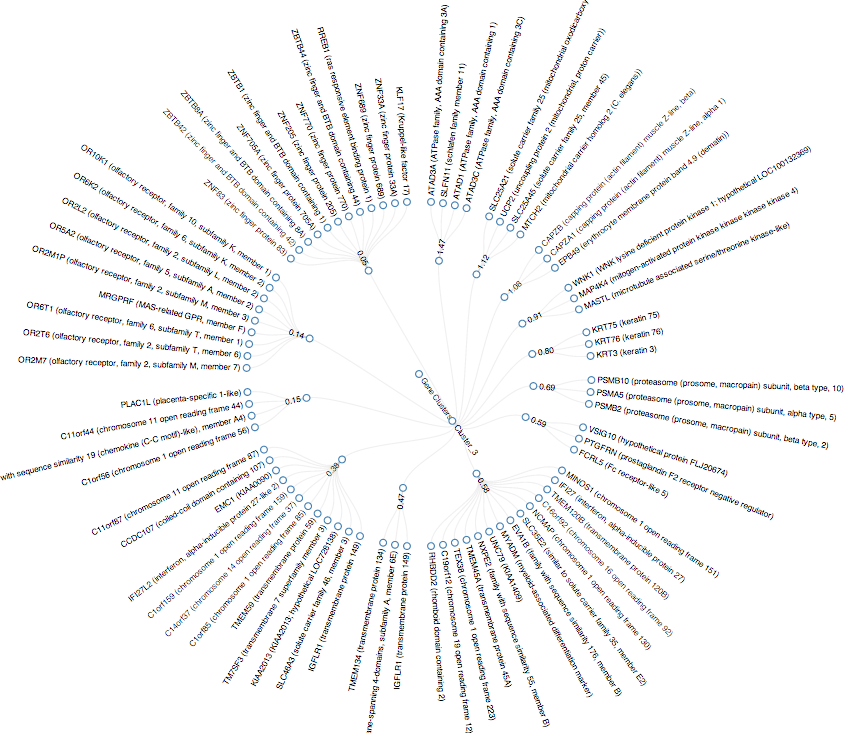
\includegraphics[width=.9\textwidth]{dendrogram.png}
    \label{fig:dendrogram}
  \end{subfigure}%

  \begin{subfigure}[b]{0.5\textwidth}
    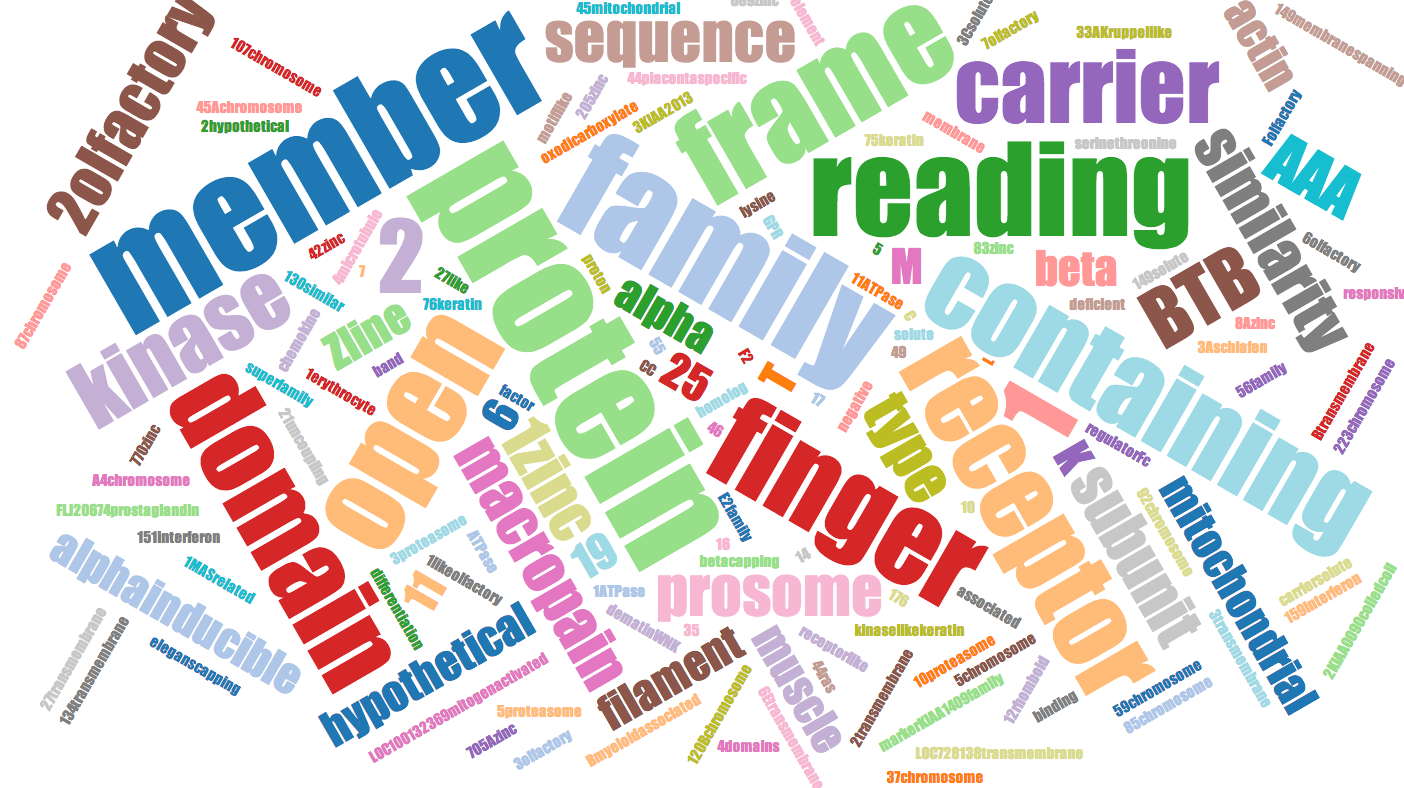
\includegraphics[width=.7\textwidth]{wordcloud.png}
    \label{fig:wordcloud}
  \end{subfigure}%
  ~
  \begin{subfigure}[b]{0.5\textwidth}
    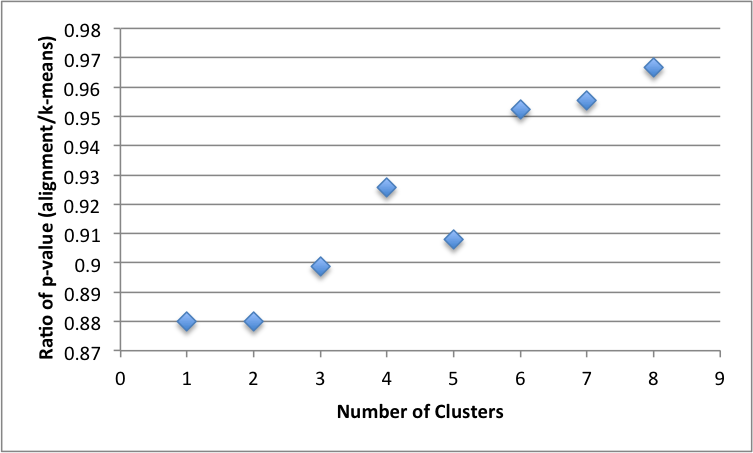
\includegraphics[width=.5\textwidth]{pvalue_performace.png}
    \label{fig:pvalue}
  \end{subfigure}%
  \label{fig:enrichment}
  \caption{A) The visualizer for gene expression. B) Dendrogram describing a cluster using our visualization tool. C) A word cloud generated from the clusters in the dendrogram. D) To give some performance metric, we took the ratio of the p-values for enrichment analysis for our technique over using plain k-means for the GSE675 dataset.}
\end{figure}


\subsection{Visualization}

In order to make the expression trend analysis easier from a clinical standpoint, we created a browser-based visualization tool (Fig.4) using \verb!d3! that provides normalized/denormalized expression trends by cluster, dendrograms for cluster annotation, and word clouds for a text summary of \verb!DAVID! gene groups by cluster.

\section{Future Goals}
We would redo the analysis on GSE33029 dataset , to identify the root cause of clusters not showing corresponding enrichment results. 

We could integrate this with the SMART Genomics API to make our tool usable for all time series of gene expression.

\section{Acknowledgements}
Thanks to Peter Szolovits, Gil Alterovitz, and Gerald Quon for their help on our project.

\begin{thebibliography} {0}

\bibitem{Snyder} Chen R, Mias G I, Li-Pook-Than J, Jiang L, et al (2012). Personal Omics profiling reveals dynamic molecular and medical phenotypes. Cell 148, 1293-1307.

\bibitem{Gerald} Gerald Quon.

\bibitem{DAVID} Huang DW, Sherman BT, Lempicki RA (2009). Systematic and integrative analysis of large gene lists using DAVID Bioinformatics Resources. Nature Protoc 4(1), 44-57.

\bibitem{webservice} Huang DW, Sherman BT, Lempicki RA (2009). Bioinformatics enrichment tools: paths toward the comprehensive functional analysis of large gene lists. Nucleic Acids Res. 37(1), 1-13.

\bibitem{GSE675} Browne EP, Wing B, Coleman D, Shenk T. Altered cellular mRNA levels in human cytomegalovirus-infected fibroblasts: viral block to the accumulation of antiviral mRNAs. J Virol 2001 Dec;75(24):12319-30. PMID: 11711622


\end{thebibliography}

\end{document}
